\section{SAT of $\hsDhom$\ over finite linear orders}\label{sec:decidability}

In this section, we devise a SAT checking procedure for $\hsDhom$ formulas over finite linear orders, which will also allow us to easily derive a MC algorithm for $\hsDhom${} over finite Kripke structures.

To start with, we show that there is a ternary relation between $\varphi$-atoms, that we denote by $\genDphi$, such that if it holds among all atoms in consecutive positions of a compass $\varphi$-structure, then the structure is fulfilling. Hence, we may say that $\genDphi$ is the rule for labeling fulfilling compasses. 

Next, we introduce an equivalence relation $\sim$ between \emph{rows} of a compass $\varphi$-structure. Since it has finite index---exponentially bounded by $|\varphi|$---and it preserves fulfillment of compasses, it is intuitively possible to ``contract'' the structures when we can find two related rows. Moreover, any contraction done according to $\sim$ keeps the same atoms (only the number of their occurrences may vary), and thus if a compass features $\varphi$ before the contraction, then $\varphi$ is still featured after it. This fact is exploited to build a SAT algorithm for $\hsDhom$ formulas which makes use of \emph{polynomial working space}, because $(i)$~it only needs to keep track of two rows of a compass at a time, $(ii)$~all rows satisfy some nice properties that make it possible to succinctly encode them, and $(iii)$~compass contractions are implicitly performed by means of a reachability check in a suitable graph, whose nodes are the equivalence classes of $\sim$.

Let us now introduce the aforementioned ternary relation $\genDphi$ among atoms.
\begin{definition}\label{def:d_generator}
Given three $\varphi$-atoms $A_1, A_2$ and $A_3$, we say that 
$A_3$ is $\Dphi$-generated by $A_1, A_2$,
written $A_1A_2\genDphi A_3$, if:  
\begin{itemize}
    \item $A_3\cap\AP = A_1 \cap A_2 \cap \AP$ and 
    \item $\reqD(A_3)=\reqD(A_1)\cup \reqD(A_2) \cup \obsD(A_1 )\cup \obsD (A_2)$.
\end{itemize}
\end{definition}


 %We will prove interesting properties related to homogeneous compass structures using  $\genDphi$. First we prove the following little property. 
%
%\begin{lemma}\label{lem:gen_implies_d}
%Given three $\varphi$-atoms $A_1, A_2$ and $A_3$  such that  
%$A_1A_2\genDphi A_3$ then  
%$A_3 \Dphi A_1$ and $A_3\Dphi A_2$.
%\end{lemma}
%\begin{proof}%PROVA OMETTIBILE
%From the definition of $\D\psi$ we have to prove that 
%for every $\BD \psi \in A_3$ we have $\{\BD \psi , \psi\}\in A_1 \cap A_2$.
%Let  $\BD \psi \in A_3$ since  $\BD \psi = \neg \D\neg \psi $
%we have $\neg \psi \notin \reqD(A_3)$. By Definition \ref{def:d_generator} 
%we have $\reqD(A_3)=\reqD(A_1)\cup \reqD(A_2) \cup \obsD(A_1 )\cup \obsD (A_2)$
%and thus $\neg \psi \notin \reqD(A_1)\cup \reqD(A_2) \cup \obsD(A_1 )\cup \obsD (A_2)$
%which means that $\neg \psi \notin \reqD(A_1)\cup \reqD(A_2)$ implies  $\BD \psi \in A_1 \cap A_2$ and $\neg \psi \notin\obsD(A_1 )\cup \obsD (A_2)$
%implies $\psi \in A_1\cap A_2$. We can conclude that $A_3 \Dphi A_1$ and $A_3\Dphi A_2$.
%\end{proof}

It is immediate to show that $A_1A_2\genDphi A_3$ if and only if $A_2A_1\genDphi A_3$ (i.e., the order of the first two components in the ternary relation is irrelevant). 
Notice that the first point of the definition enforces the homogeneity assumption.

The next result, immediately following from Proposition~\ref{prop:unique}, proves that $\genDphi$ expresses a \emph{functional dependency} on $\varphi$-atoms.
%
\begin{lemma}\label{lem:functional}
Given two $\varphi$-atoms $A_1, A_2\in \Atoms$, there exists \emph{exactly one} $\varphi$-atom  $A_3\in \Atoms$  such that $A_1A_2\genDphi A_3$.
\end{lemma}
%
% \begin{proof} 
% Let us suppose by contradiction that there exist $A_3$ and $A_3'$ in $\Atoms$ such that $A_3\neq A_3'$, $A_1A_2\genDphi A_3$ and  $A_1A_2\genDphi A_3'$.
% By Definition \ref{def:d-atom} we  can assume w.l.o.g.\ that there exists $\psi\in \CL(\varphi)$ such that $\psi \in A_3$ and $\neg \psi \in A_3'$.
% Moreover we choose $\psi$ as a minimal formula that satisfies $\psi \in A_3$ and $\neg \psi \in A_3'$, i.e.,
% each proper sub-formula $\psi'$ of $\psi$ either belongs to both $A_3$ and $A_3'$ or does not belong to either 
% $A_3$ or $A_3'$.

% Let us now prove that we get a contradiction.
% If $\psi=p$, with $p\in \AP$, by Definition~\ref{def:d_generator} $A_3\cap\AP = A_1 \cap A_2 \cap \AP $ and thus $p \in A_1\cap A_2\cap \AP $; since $A_3'\cap\AP = A_1 \cap A_2 \cap \AP $,
% we have $p\in A_3'$. Hence, both $p$ and $\neg p$ belong to $A_3'$ which contradicts Definition~\ref{def:d-atom}.

% If $\psi=\neg \psi_1$, by the minimality of $\psi$,
% either $\psi_1\in A_3\cap A_3'$ or $\psi_1\notin A_3\cup A_3'$.
% In the former case we have $\neg \psi_1, \psi_1\in A_3$ (contradiction).
% As for the latter, since we are assuming $\neg \psi\in A_3'$, we have $\neg \neg \psi_1\in A_3'$,
% i.e., $\psi_1\in A_3'$ (contradiction).

% If $\psi= \psi_1 \vee \psi_2 $, let us consider w.l.o.g.\ the case in which 
% $\psi_1 \in A_3$. Since $\neg (\psi_1 \vee \psi_2)\in A_3'$ we have $\neg \psi_1 \in A_3'$
% and thus $\psi_1 \notin A_3'$. However, 
% by the minimality of $\psi$  and since $\psi_1 \in A_3$, we have that 
% $\psi_1\in A_3'$ (contradiction). 

% Finally,
% if $\psi=\D \psi_1$
% then $\neg \D \psi_1 \in A_3'$, hence $\psi_1\notin \reqD(A_3')=\reqD(A_1)\cup \reqD(A_2) \cup \obsD(A_1 )\cup \obsD (A_2)$. Since $\psi \in A_3$ we have $\psi_1\in \reqD(A_3)= \reqD(A_1)\cup \reqD(A_2) \cup \obsD(A_1 )\cup \obsD (A_2)$ (contradiction). 
% \end{proof}

Definition~\ref{def:d_generator} and Lemma~\ref{lem:functional} can be exploited to label a homogeneous compass $\varphi$-structure $\cG$, namely, to determine the $\varphi$-atoms labeling all the points $(x,y)$ of $\cG$, starting from the ones on the diagonal.
The idea is the following: if two $\varphi$-atoms $A_1$ and $A_2$ label respectively the greatest proper prefix $[x,y-1]$, that is, the point $(x,y-1)$, and the greatest proper suffix $[x+1,y]$, that is, $(x+1,y)$, of the same interval $[x,y]$,  
then the atom $A_3$ labeling $[x,y]$ is unique, and it is precisely the one satisfying $A_1A_2\genDphi A_3$ (see Figure~\ref{fig:labelling}). The next lemma, proved in Appendix~\ref{proof:lem:compass_hom_gen}, claims that this is the general rule for labeling fulfilling homogeneous compasses.

\begin{figure}[tb]
    %\vspace*{-0.2cm}
    \centering
    \begin{tikzpicture}[scale=0.8]

\draw[step=1cm,gray, thin] (-3,-3) grid (3,3);

\draw (-3,-3) -- (3,3);
\fill[color=white] (-3,-3) node (v1) {} -- (3.1,3.1) -- (3.1,-3);

\draw [-latex](-3,-3) -- (4,-3);
\draw [-latex](-3,-3) -- (-3,4);

\draw[thick,- triangle 90, decorate, decoration=zigzag] (2,2) -- (-3,2);
\draw[thick,- triangle 90, decorate, decoration=zigzag] (1,1) -- (-3,1);

\node[draw,circle,fill=lightgray] (v3) at (-1,2) {};
\node[draw,circle,fill=lightgray] (v2) at (-1,1) {};
\node[draw,circle,fill=lightgray] (v4) at (0,2) {};

%\draw [-stealth] plot[smooth, tension=.7] coordinates {(v2.north east) (-0.5,1.5) (v3.south east)};
%\draw [-stealth] plot[smooth, tension=.7] coordinates {(v4.north west) (-0.5,2.5) (v3.north east)};

\node (v6) at (-1.5,4) {$(x,y)$};
\node (v5) at (0.5,4) {$(x\!+\!1,y)$};
\node (v7) at (1.8,-0.3) {$(x,y\!-\! 1)$};

\draw [dashed](-1,-1) -- (-1,-3);
\draw [dashed](0,0) -- (0,-3);

\node at (-1,-3.5) {$x$};
\node at (0,-3.5) {$x\!+\!1$};
\node at (-3.5,2) {$y$};
\node at (-3.5,1) {$y\!-\! 1$};

\node at (2,0.9) {$row_{y - 1}$};
\node at (2.8,1.9) {$row_y$};

\draw [gray] (v5) edge (v4);
\draw [gray] (v6) edge (v3);
\draw [gray] (v7.west) edge (v2);

\draw [red,ultra thick,<-] (v3) edge (v2);
\draw [red,ultra thick,<-] (v3) edge (v4);
\end{tikzpicture}
    %\vspace{0.2cm}
    \caption{Rule for labeling homogeneous fulfilling compass $\varphi$-structures}
    \label{fig:labelling}
\end{figure}

\begin{lemma}\label{lem:compass_hom_gen}
Let $\cG=(\bbP_\bbD,\cL)$. $\cG$ is a fulfilling homogeneous compass $\varphi$-structure if and only if, for every pair $x,y \in \mathpzc{S}$,  we have: 
\begin{itemize}
    \item $\cL(x,y-1)\cL(x+1, y)\genDphi \cL(x, y)$ if $x<y$, and 
    \item $\reqD(\cL(x,y))=\emptyset$ if $x=y$.
\end{itemize}
\end{lemma}
%



%The contrapositive implication of Lemma \ref{lem:compass_hom_gen} states that, given a homogeneous compass $\varphi$-structure $\cG=(\bbP_\bbD,\cL)$, if in some point $(x,y)\in\bbP_\bbD$ with $x<y$, $\cL(x,y-1)\cL(x+1, y)\genDphi \cL(x, y)$ \emph{does not} hold, then $\cG$ is \emph{not} fulfilling. Therefore, in order to decide whether a \hsD -formula $\varphi$ is satisfiable, we will have to apply $\genDphi$ everywhere in a (any) compass $\varphi$-structure, while generating it.

Now we introduce the concept of $\varphi$-row, which can be viewed as the ordered sequence of (the occurrences of) atoms labelling a row of a compass $\varphi$-structure. Given an atom $A \in \Atoms$, we call it \emph{reflexive} if 
$A \Dphi A$, and \emph{irreflexive} otherwise.
%
\begin{definition}\label{def:row}
A $\varphi$-row is a finite sequence of $\varphi$-atoms \[\row=A_0^{m_0}\cdots A_n^{m_n},\] where $A^m$ stands for $m$ repetitions of $A$, such that for each $0\leq i \leq n$, we have that $m_i>0$---if $m_i>1$, then $A_i$ is reflexive---and for each $0\leq j<i$, it holds that $A_i \Dphi A_j$,  $A_i \neq A_j$, and $(A_j\cap \AP)\supseteq (A_i\cap \AP)$. Moreover, $\reqD(A_0)=\emptyset$.
\end{definition}

The length of a $\varphi$-row $\row=A_0^{m_0} \cdots A_n^{m_n}$ is defined as $|\row|=\sum_{0\leq i \leq n} m_i$, and for each $0\leq j<|\row|$, the $j$-th element, denoted by $\row(j)$, is the $j$-th symbol in the word $A_0^{m_0} \cdots A_n^{m_n}$, e.g., $\row(0)=A_0$, $\row(m_0)=A_1$, \dots; finally
$\row(i, j)$, for  $0\leq i \leq j < |\row|$, represents the sub-word $\row(i)\row(i+1)\cdots \row(j)$.
We denote by $\Rows$ the set of all possible $\varphi$-rows. This set may be infinite.

The number of distinct atoms in any $\varphi$-row is bounded. 
Since for each $0\leq i \leq n$ and each $0\leq j<i$, $A_i \Dphi A_j$,
it holds that $\reqD(A_j) \subseteq \reqD(A_i)$.  
Therefore, two monotonic sequences for every 
$\varphi$-row can be considered, one increasing, i.e., $\emptyset=\reqD(A_0) \subseteq \reqD(A_1)\subseteq \ldots \subseteq \reqD(A_n)$,
and one decreasing, i.e., $(A_0 \cap \AP)\supseteq (A_1\cap \AP)\supseteq \ldots \supseteq (A_n\cap \AP)$. 
The number of distinct elements is bounded by $|\varphi|$ in the former sequence and by $|\varphi|+1$ in the latter (as $|\REQ_{\varphi}|\leq |\varphi|-1$ and $|\AP|\leq |\varphi|$--w.l.o.g., we can consider only the letters actually occurring in $\varphi$). Since, as already shown (Proposition~\ref{prop:unique}), a set of requests and a set of proposition letters uniquely determine a $\varphi$-atom, any $\varphi$-row may feature at most $2|\varphi|$ distinct atoms, namely, $n<2|\varphi|$.  

Given a homogeneous compass $\varphi$-structure $\cG= (\bbP_\bbD,\cL)$, for every  $y\in \mathpzc{S}$, we define $\row_y$ as the word of $\varphi$-atoms $\row_y=\cL(y,y)\cdots \cL(0, y)$, i.e., the sequence of atoms labeling points of $\cG$ with the same $y$-coordinate, starting from the one on the diagonal \emph{inwards}. See Figure~\ref{fig:labelling}. 

The next result holds; its proof can be found in Appendix~\ref{proof:lem:compas_implies_row}.
\begin{lemma}\label{lem:compas_implies_row}
Let $\cG= (\bbP_\bbD,\cL)$ be a fulfilling homogeneous compass $\varphi$-structure. For every $y\in \mathpzc{S}$, $\row_y$ is a $\varphi$-row.
\end{lemma}
%

We now define the \emph{successor} relation between pairs of $\varphi$-rows, denoted as $\rownext$, which is basically a component-wise application of $\genDphi$ over the elements of two $\varphi$-rows (remember that atoms on rows are collected right-to-left).
%
\begin{definition}\label{def:rownext}
Given two $\varphi$-rows $\row$ and $\row'$, we say that $\row'$ is a \emph{successor}
of $\row$, written as $\row \rownext \row'$, if $|\row'| = |\row| +1$, and for all $0\leq i < |\row|$,
$\row(i)\row'(i) \genDphi \row'(i+1)$. 
\end{definition}

The next lemma, whose proof is in Appendix~\ref{proof:lem:row_successor}, states that consecutive  rows in homogeneous fulfilling compass $\varphi$-structures respect the successor relation.
%
\begin{lemma}\label{lem:row_successor}
Let $\cG=(\bbP_\bbD,\cL)$, with $\reqD(\cL(x,x))=\emptyset$ for all $(x,x)\in\bbP_\bbD$. $\cG$ is a fulfilling homogeneous compass $\varphi$-structure
if and only if, for each $0\leq y < |\mathpzc{S}| -1$, $\row_y \rownext \row_{y+1}$.
\end{lemma}
%


Given an atom $A \in \Atoms$, we define the \emph{rank of $A$}, written $\rank(A)$, as %the number $\rank(A)= 
$|\REQ_\varphi| - |\reqD(A)|$.  Clearly, $\rank(A)< |\varphi|$. Whenever $A \Dphi A'$, for some $A' \in \Atoms$, $\reqD(A')\subseteq \reqD(A)$, and thus  $\rank(A)\leq \rank(A')$ and $|\reqD(A)\setminus \reqD(A')|\leq \rank(A')$.
%For this reason, 
We can see the $\rank$ of an atom as the ``number of degrees of freedom'' 
that it gives to %imposes on
the atoms  that stay ``above it''.
In particular, by definition, for every $\varphi$-row $\row=A_0^{m_0} \cdots A_n^{m_n}$, we have $\rank(A_0)\geq \ldots \geq  \rank(A_n)$.
%
The next lemmas use the notion of rank to provide an insight on how consecutive $\varphi$-rows are connected
(see Figure~\ref{fig:rank}).

\begin{figure}[tb]
    \centering
    \resizebox{\linewidth}{!}{\begin{tikzpicture}

\node[inner sep=0pt, label={[label distance=0.3cm]180:$\row_1$}](R1A) {\phantom{$A$}};
\node[inner sep=0pt, right of=R1A](R1B) {\phantom{$A$}};
\node[fit=(R1A)(R1B), draw, fill=gray!50] (R1){};
 \fill[pattern=north east lines] (R1.north west) rectangle (R1.south east);

\node(AMI)[draw, rounded corners, right of=R1B,node distance=0.8cm]{$A_i$};
\node(AD)[right of=AMI,node distance=1.8cm]{$\ldots\quad${\huge $\uparrow$}$k\quad\ldots$};
\node(A1)[draw, rounded corners,right of=AD,node distance=2.5cm]{$A_i$};

\node(BJ)[draw, label={[label distance=-0.6cm]0:$B'$}, rounded corners,above of=A1,node distance=0.9cm]{$\phantom{A_i}$};
\node(BJ1)[draw , label={[label distance=-0.7cm]0:$B''$},rounded corners,left of=BJ,node distance=0.9cm]{$\phantom{A_i}$};
\node(BD)[left of=BJ1,node distance=0.6cm]{$\ldots$};
\node(BJ1K)[draw , label={[label distance=-0.7cm]0:$B'''$},rounded corners,left of=BD,node distance=1.1cm]{$\phantom{A_i}$};
\node(BD)[left of=BJ1K,node distance=0.6cm]{$\ldots$};
\node(BJ1KE)[draw , label={[label distance=-0.7cm]0:$B'''$},rounded corners,left of=BD,node distance=1.1cm]{$\phantom{A_i}$};
\draw[decorate, decoration={brace, raise=0.4cm, amplitude=0.25cm}, line width=0.3mm] (BJ1KE.west) -- (BJ1K.east)node[pos=0.5, above, yshift=0.6cm]{$=$};

\node[inner sep=0pt, label={[label distance=0.3cm]180:$ $}](R11A) [right of=A1] {\phantom{$A$}};
\node[inner sep=0pt, right of=R11A](R11B) {\phantom{$A$}};
\node[fit=(R11A)(R11B), draw, fill=gray!50] (R11){};
 \fill[pattern=north east lines] (R11.north west) rectangle (R11.south east);

\node(SB)[draw, rounded corners,node distance=0.8cm, fill=gray!50] [above of=R11A, node distance=0.9cm]{$\phantom{A_i}$};
 \fill[pattern=north east lines] (SB.north west) rectangle (SB.south east);

\node[inner sep=0pt, label={[label distance=0.3cm]180:$ $}](R21A) [right of=SB, node distance=0.7cm] {\phantom{$A$}};
\node[inner sep=0pt, right of=R21A](R21B) {\phantom{$A$}};

\node[inner sep=0pt, label={[label distance=0.3cm]180:$\row_2$}](R2A) [above of=R1A, node distance=1cm] {\phantom{$A$}};
\node[inner sep=0pt, right of=R2A](R2B) {\phantom{$A$}};
\node[fit=(R2A)(R2B), draw, fill=gray!50] (R2){};
 \fill[pattern=north east lines] (R2.north west) rectangle (R2.south east);
\node[fit=(R21A)(R21B), draw, fill=gray!50] (R21){};
 \fill[pattern=north east lines] (R21.north west) rectangle (R21.south east);


\draw[decorate, decoration={brace, mirror, raise=0.4cm, amplitude=0.25cm}, line width=0.3mm] (AMI.west) -- (A1.east)node[pos=0.5, below, yshift=-0.7cm]{$m_i$};

\path let
         \p1 = ($(SB.north east)-(A1.south west)+(1,0)$),
         \n1 = {veclen(\p1)}
         in
         (SB.south) -- (A1.north) 
         node[midway, sloped, draw, red, ellipse, line width=0.4mm,
          minimum width=\n1/1.29, rotate=18, minimum height=\n1/3.2, xshift=0.0cm, yshift=0.03cm](STARTS) {};
\node(STARTS_L)[above right of=STARTS, yshift=0.5cm, xshift=1.5cm, draw, line width=0.4mm, red]{$start_i$ positions};
\draw[red, line width=0.4mm] (STARTS) -- (STARTS_L.south west);
\pgftransformshift{\pgfpoint{4cm}{-1.5cm}}
\node{$\begin{array}{c}
rank(A_i)\geq rank(B')> rank(B'') > \ldots > rank(B''') 
\end{array}$};
\pgftransformshift{\pgfpoint{7cm}{1.5cm}}
\node{$\begin{array}{c}
B' = \row_2(start_i+1)\end{array}$};
\end{tikzpicture}}
    %\vspace*{-0.1cm}
\caption{A graphical account of the proof of Lemma~\ref{lem:rank}}\label{fig:rank}
\end{figure}

\begin{lemma}\label{lem:rank0}
Let $\row_1$ and $\row_2$ be two $\varphi$-rows, with
$\row_1= A_0^{m_0}\cdots A_n^{m_n}$ and $\row_1\rownext \row_2$. 
For each $0\leq i\leq n$, let $st_i=\sum_{0\leq j <i} m_j$.
If, for some $st_i<j\leq st_i + m_i $, the atom $\row_2(j)$ is reflexive, then 
for each $j\leq j'\leq st_i + m_i$, $\row_2(j')=\row_2(j)$.
\end{lemma}
\begin{proof}
If $j=st_i+m_i$ there is nothing to prove. Thus we consider $j<st_i+m_i$.
Since $\row_2(j)$ is reflexive,   
$\obsD(\row_2(j))\subseteq \reqD(\row_2(j)) $. %=\obsD(\row_2[j-1])\cup \reqD(\row_2[j-1])\cup\obsD(A_i)\cup\reqD(A_i)=
%\obsD(\row_2[j-1])\cup \reqD(\row_2[j-1])\cup\reqD(A_i)
%$,
%because $A_i$ is reflexive and $\row_1 \rownext \row_2 $.
%
Since $\row_1 \rownext \row_2 $, we have that $\reqD(A_i),\obsD(A_i)\subseteq\reqD(\row_2(j))$ %since $A_i$ is reflexive $\reqD(A_i)\supseteq\obsD(A_i)$.
and $\reqD(\row_2(j+1))=\reqD(\row_2(j))\cup\obsD(\row_2(j))\cup\reqD(A_i)\cup\obsD(A_i)=\reqD(\row_2(j))$.
%
Moreover, from $\row_1 \rownext \row_2 $, we have $\row_2(j)\cap \AP = \row_2(j-1) \cap A_i\cap \AP$ and $\row_2(j+1)\cap \AP = \row_2(j) \cap A_i\cap \AP=\row_2(j-1) \cap A_i\cap \AP$. 
Thus, $\row_2(j+1) = \row_2(j)$, because the two atoms feature exactly the same requests and proposition letters (Proposition~\ref{prop:unique}).
Then,
since $A_i \ \row_2(j)\genDphi \row_2(j+1)$, 
% have that $\reqD(\row_2[j])= \reqD(A_i)\cup \reqD(\row_2[j-1]) \cup \obsD(A_i) \cup \obsD(\row_2[j-1])=
% \reqD(\row_2[j]) \cup \obsD(A_i) \cup \obsD(\row_2[j])$
% and $\row_2[j])\cap A_i\cap \AP = \row_2[j-1])\cap A_i\cap \AP$ from Lemma \ref{lem:functional}
% can conclude that
%$A_i \row_2[j] \genDphi \row_2[j]$ by Lemma \ref{lem:functional} and thus $ \row_2[j] = \row_2[j+1]$. 
by iterating the reasoning and exploiting Lemma~\ref{lem:functional}, we can conclude that
$\row_2(j)=\row_2(j')$ for each $j\leq j'\leq st_i + m_i$.
\end{proof}

\begin{lemma}\label{lem:rank}
Let $\row_1$ and $\row_2$ be two $\varphi$-rows, with
$\row_1= A_0^{m_0}\cdots A_n^{m_n}$ and $\row_1\rownext \row_2$. 
For each $0\leq i\leq n$, let $st_i=\sum_{0\leq j <i} m_j$.
If $m_i > rank(A_i)$, then there exists $st_i<k\leq st_i + m_i $
such that:
\begin{itemize}
\item $k\leq st_i+1+\rank(A_i)$;
\item $\row_2(k)$ is reflexive;
\item $\rank(\row_2(j))>\rank(\row_2(j+1))$ for each $st_i<j< k$; 
\item $\row_2(j)=\row_2(j+1)$ for each $k \leq j< st_i + m_i$;
\item if $m'$ is the exponent of the atom $\row_2(k)$ in $\row_2(st_i+1, st_i+m_i)$ then  $m'>  \rank(\row_2(k)) $.
\end{itemize}
\end{lemma}
\begin{proof}
%
If $m_i=1$, by hypothesis we have $ rank(A_i) = 0$. Hence, $rank(\row_2(st_i+1)) = 0$, because $\row_1\rownext \row_2$, and thus $\row_2(st_i+1)$ is (trivially) reflexive. All claims hold by choosing $k=st_i+1$. 

Let us then assume $m_i>1$. %, hence $A_i$ is reflexive.
It can be easily shown that if we have two atoms $A$ and $A'$ such that $A\Dphi A'$ and $A'$ is irreflexive, then $rank(A)< rank(A')$.
Moreover, Lemma \ref{lem:rank0} proves that we cannot interleave reflexive atoms with irreflexive ones ``above'' the $A_i$'s (i.e., all irreflexive atoms must ``come before'' reflexive ones in the part of $row_2$ ``above'' the $A_i$'s).
Thus, in the worst case, the atoms $\row_2(st_i+1),\ldots ,\row_2(st_i+rank(A_i))$
may be irreflexive (as $rank(\row_2(st_i+1))>\ldots >rank(\row_2(st_i+rank(A_i)))$ and $rank(A_i)\geq rank(\row_2(st_i+1))$). Note that these irreflexive atoms may be the ``first''  $rank(A_i)$
atoms above the $A_i$'s only, and not the ``first'' $rank(A_i)+1$,
since any atom with rank equal to $0$ is reflexive. 
% Moreover,
% for every $0<j< m_i$ if $\row_2(st_i+j)$ is irreflelexive then 
% $rank(\row_2(st_i+j))> \row_2(st_i+j+1)$.
%
We conclude that $\row_2(st_i+rank(A_i)+1)$ must be reflexive. %(and it is still an atom ``above`` $A_i$, since $m_i \geq rank(A_i)+1$ by hypothesis). 
Thus, we can choose $k=st_i+rank(A_i)+1$. Since by hypothesis $m_i\geq rank(A_i)+1$, we get that
$st_i<k\leq st_i+m_i$. Finally, by Lemma \ref{lem:rank0}, $\row_2(j)=\row_2(j+1)$ for each $k \leq j< st_i + m_i$.

As for the last claim,  we have $rank(row_2(k))\leq rank(row_2(st_i+1)) - (k - st_i -1) \leq rank(A_i) - (k - st_i -1)$. 
Then, the exponent $m'$ of $row_2(k)$ in $\row_2(st_i+1, st_i+m_i)$ is such that
$m'\geq m_i - (rank(A_i) - rank(\row_2(k)))$,
that is, at least $m_i - (rank(A_i) - rank(\row_2(k)))$ atoms 
labelled by $\row_2(k)$ occur in the block $st_i+1,\ldots, st_i + m_i$  
of $\row_2$ (see Figure~\ref{fig:rank}). 
% Then 
% and thus we have  $m_i - rank(A_i) + rank(\row_2(k)) \leq m'$.
Since by hypothesis $m_i>rank(A_i)$, then $m_i-rank(A_i)>0$ and 
$rank(\row_2(k)) < m'$.
\end{proof}

% \begin{proof} %% PROVA NON OMETTIBILE ATTENZIONE NON OMETTIBILE :D:D:D
% Since the rank is  monotone non-increasing along the row,
% $\rank(\row_2[start_i+1])\geq \ldots\geq \rank(\row_2[start_i +m_i])$.
% Let us assume by contradiction that there exists $start_i<k_1<k_1+1<\ldots<k_2-1<k_2\leq start_i +m_i$
% such that $\rank(\row_2[k_1])>\rank(\row_2[k_1+1])=\ldots=\rank(\row_2[k_2-1])>\rank(\row_2[k_2])$. 
% Since $\row_1\rownext \row_2$, we have  $\row_1[start_i+j]\row_2[start_i+j]\genDphi \row_2[start_i+j+1]$
% for every $0 \leq j < m_i$. By Definition~\ref{def:rownext} and the fact that 
% $\row_1[start_i+j]= \row_1[start_i+j+1]$ for every $0 \leq j < m_i$, we get 
% $\row_2[start_i+j]\cap \AP = \row_2[start_i+j+1]\cap \AP$, $0 < j \leq m_i$.
% Since $\row_1[k_1+1]\row_2[k_1+1]\genDphi \row_2[k_1+2]$, we have that
% $\reqD(\row_2[k_1+2])=\reqD(\row_1[k_1+1])$  
% and $\row_2[k_1+2])\cap \AP=\row_1[k_1+1] \cap \AP$.
% We can conclude that $\row_2[k_1+1] = \row_2[k_1+2]$, as the set of requests and the set of proposition letters
% uniquely determine a $\varphi$-atom. Since $ \row_1[k_1+j]$ do not change 
% for every $start_i \leq j < m_i$, we have that $\row_2[k_2-1]= \row_2[k_2]$,  which is a contradiction
% because $\rank(\row_2[k_2-1])>\rank(\row_2[k_2])$ (i.e., $\row_2[k_2]$ is supposed to be equal to  $\row_2[k_2-1]$ with a different rank). As for the 
% second point, we have proved above that we have $k$ consecutive increasing in rank and then a $m_i-k$ long sequence of atoms
% identical to  $\row_2[k]$ hypothesis immediately follows.
% \end{proof}
%\begin{proof}
%By hypothesis, $(i)$ $row_1[start_i]=\ldots = %row_1[start_i+m_i-1]=A_i$, and $(ii)$ $row_1[start_i+j] %row_2[start_i+j]\genDphi row_2[start_i+j+1]$ for all $0\leq %j< m_i$. 
%As a consequence, we easily get $row_2[start_i+1]\cap\AP=\ldots = row_2[start_i+m_i]\cap\AP$. 
%Moreover, by Lemma~\ref{lem:transitive_req}, $\reqD(row_2[t]) \subseteq\reqD(row_2[t+1])$ for all $0\leq t<|row_2|$, hence $(iii)$ $\rank(row_2[t]) \geq \rank(row_2[t+1])$.
%
%Let us now consider (if it exists) the \emph{minimal} index %$1\leq k< m_i$
%for which we have $row_2[start_i+k]=row_2[start_i+k+1]$; by Lemma~\ref{lem:functional} and $(ii)$, we get $row_2[start_i+k]=\ldots = row_2[start_i+m_i]$. Therefore by $(iii)$ we can assume w.l.o.g.\ that $\rank(row_2[start_i+1])> \ldots > \rank(row_2[start_i+k])$.
%Since $row_1[start_i] row_2[start_i]\genDphi row_2[start_i+1]$, we have that $\reqD(row_1[start_i])\subseteq\reqD(row_2[start_i+1])$, hence $\rank(A_i)=\rank(row_1[start_i])\geq\rank(row_2[start_i+1])$. Since we are assuming \underline{$m_i\geq rank(A_i)+2$}, such a $k$ has to exist, and $k\leq\rank(A_i)+1$.
%\end{proof}

Now we introduce an equivalence relation $\sim$ over $\Rows$ which is the key ingredient of the proofs showing that 
both SAT and MC for $\hsDhom$ formulas are decidable.
%
\begin{definition}\label{def:equivalence_class}
Given two $\varphi$-rows $\row_1=A_0^{m_0} \cdots A_n^{m_n}$ and $\row_2=
\hA_0^{\hm_0} \cdots \hA_{\hn}^{\hm_{\hn}}$, we say that they are \emph{equivalent}, written 
$\row_1 \sim \row_2$,
if 
\begin{itemize}
    \item $n=\hn$, and 
    \item for each $0\leq i \leq n$, $A_i =\hA_i$, and ${m_i=\hm_i}$ or
    both $m_i$ and $\hm_i$ are (strictly) greater than $\rank(A_i)$.
\end{itemize}
\end{definition}
%
Note that if two rows feature the same set of atoms, the lower the rank of an atom 
$A_i$, the lower the number of occurrences of $A_i$ both the rows have to feature in order to belong to the same equivalence class.
As an example, let $\row_1$ and $\row_2$ be two rows with $\row_1=A_0^{m_0}A_1^{m_1}$,
$\row_2=A_0^{\om_0}A_1^{\om_1}$, $\rank(A_0) = 4$, 
and $\rank(A_1)= 3$. If $m_1 = 4$ and $\om_1=5$, they are both greater than $\rank(A_1)$, and
thus they do not violate the condition for $\row_1 \sim \row_2$. On the other hand,
if $m_0 = 4$ and $\om_0=5$, we have that $m_0$  is less than or equal to $\rank(A_0)$. Thus, in this case, $\row_1 \not\sim \row_2$ due to the indexes of $A_0$. This happens because $\rank(A_0)$ is greater than $\rank(A_1)$. Two cases in which $\row_1 \sim \row_2$ 
are $m_0 = \om_0$ and $m_0, \om_0 \geq 5$. 
%Defining equivalence classes 
%this way turns out to be crucial for proving our result and for constructing an automaton that 
%recognizes the language of $\varphi$.

The relation $\sim$ has finite index, which is roughly bounded  by  the number of  all the possible $\varphi$-rows $\row=A_0^{m_0}\cdots A_n^{m_n}$, with exponents $m_i$ ranging from  $1$ to $ |\varphi|$. Since $(i)$~the number of possible atoms is $2^{|\varphi|}$, $(ii)$~the number of \emph{distinct} atoms in any $\varphi$-row is at most $2|\varphi|$, and $(iii)$~the number of possible functions
%  $ f: \{1,\ldots , 2|\varphi|\} \rightarrow \{ 1,\ldots ,|\varphi| + 1 \}$ is $(|\varphi|+1)^{2|\varphi|}= 2^{2|\varphi|\log(|
% \varphi|+1)}$, we get that the number of distinct equivalence classes of $\sim$ is bounded by 
% $2^{2|\varphi|^2} 2^{2|\varphi|\log(|\varphi|+1)}= 2^{2|\varphi| (  |\varphi| + \log(|\varphi|+1))}$, 
$f: \{1,\ldots , \ell\} \rightarrow \{ 1,\ldots ,|\varphi|\}$ is $|\varphi|^{\ell}$, we have that the number of distinct equivalence classes of $\sim$ is bounded by
\[
    \sum_{j=1}^{2|\varphi|} (2^{|\varphi|})^j\cdot |\varphi|^j\leq  2^{3|\varphi|^2},
\]
%
which is exponential in the length of the input formula 
$\varphi$. We denote the set of equivalence classes of $\sim$ over all the possible $\varphi$-rows by $\Rows^\sim$. 

Now we extend $\rownext$ to equivalence classes of $\sim$ in the following way. 
%
\begin{definition}\label{def:row_class_suc}
Given two $\varphi$-row
classes $[\row_1]_\sim$ and $[\row_2]_\sim$, we say that $[\row_2]_\sim$ is a successor of  $[\row_1]_\sim$, 
written $[\row_1]_\sim\rownext [\row_2]_\sim$, if there exist 
$\row_1' \!\in\! [\row_1]_\sim$ and $\row_2' \!\in\!  [\row_2]_\sim$ such that 
$\row_1' \rownext \row_2'$.
\end{definition}

The following fundamental result proves that if some $\row_1' \in [\row_1]_\sim$ has a successor in $[\row_2]_\sim$, %actually 
then \emph{every $\varphi$-row} of $[\row_1]_\sim$ has a successor in $[\row_2]_\sim$ (hence the definition of $\rownext$ over the equivalence classes of $\sim$ is well-given). 

%
\begin{lemma}\label{lem:row_class_suc}
Given two $\varphi$-row
classes $[\row_1]_\sim$ and $[\row_2]_\sim$ such that 
$[\row_1]_\sim\rownext [\row_2]_\sim$, \emph{for every} $\row\!\in\! [\row_1]_\sim$ there exists 
$\row'\!\in\! [\row_2]_\sim$ such that $\row\rownext \row'$.
\end{lemma}

Before starting the proof we observe that,
since $[\row_1]_\sim
\rownext [\row_2]_\sim$, 
there exists $\row \in [\row_1]_\sim$
and $\orow\in [\row_2]_\sim$ such that $\row \rownext \orow$. Thus, if $|[\row_1]_\sim|=1$, 
the lemma trivially holds. 

In the following we suppose that $|[\row_1]_\sim|\geq 2$: then there is $\row' \neq \row$ such that 
$\row' \sim \row$. We let $\row = A_0^{m_0}\cdots A_n^{m_n}$; by definition we have
$\row' =A_0^{m_0'}\cdots A_n^{m_n'}$, where for every $0\leq i \leq n$,
$m_i'= m_i$ if  $m_i\leq \rank(A_i)$, and $m_i'> \rank(A_i)$ if $m_i > \rank(A_i)$.

Hereafter, we will say that \lq\lq $A_i$ exceeds its rank in $\row$\rq\rq{}
whenever $m_i> \rank(A_i)$.
Moreover, for the sake of the proof it is worth observing that any sub-word $\row(0, i)$ is a $\varphi$-row for every $0\leq i < |\row|$, and, 
since $\row\rownext \orow$, then $\row(0, i)\rownext \orow(0, i+1)$.
 
We now want to determine 
$\orow'$ such that 
$\row' \rownext \orow' $  and $\orow'\sim \orow$, proving the lemma.
%
To this aim, we define a list of $\varphi$-rows $\orow'_{-1}, \orow'_0,\ldots ,\orow'_n$ such that
$\orow'_{-1}=\orow(0)$ and,
for all $0\leq i\leq n$, $\orow'_i$ extends $\orow'_{i-1}$; we will show that $\orow'_n=\orow'$ (i.e., the row we want to determine).

The $\varphi$-rows $\orow'_i$, for $i\geq 0$, are formally defined as:
\begin{small}
\[
\orow'_i =
\begin{cases} 
   \orow'_{i-1} \cdot \orow(st_i+1, st_i+m_i) 		& \text{if } m_i=m'_i \\
   \orow'_{i-1} \cdot \orow(st_i+1, st_i+m'_i)		& \text{if } \rank(A_i)\!<\! m'_i\!<\! m_i \\
   \orow'_{i-1} \cdot \orow(st_i+1, st_i+m_i) \cdot (\orow(st_i+m_i))^{m'_i-m_i}	& \text{if } \rank(A_i)\!<\! m_i\!<\! m'_i 
  \end{cases}
\]
\end{small}
Intuitively, if $m_i=m'_i$, $\orow'_i$ is obtained just by appending the block $\orow(st_i+1, st_i+m_i)$ to $\orow'_{i-1}$. If $\rank(A_i)<m'_i<m_i$, we do almost the same thing, but we ``truncate'' the block after $m'_i$ positions, instead of $m_i$. Finally, if $\rank(A_i)<m_i<m'_i$, then $\orow'_i$ is obtained by appending $\orow(st_i+1, st_i+m_i)$ to $\orow'_{i-1}$, with $m'_i-m_i$ additional repetitions of $\orow(st_i+m_i)$ at the end, as we need to ``pump'' $\orow'_i$ in order for it to have a suitable length with respect to $\row'$, thus respecting $\rownext$.

%\newcommand{\lst}{\mathsf{lst}}

We are now ready to prove Lemma~\ref{lem:row_class_suc}
\begin{proof}
We show that the following properties hold by induction on $0\leq i\leq n$, where 
%$\lst(\row)$ denotes the last atom of $\row$, and 
$st_i=\sum_{0\leq j <i} m_j$ and $st'_i=\sum_{0\leq j <i} m'_j$ are respectively the starting positions of $A_i$ in $\row$ and $\row'$:
\begin{enumerate}
    \item[0.] $\orow'_i$ is a $\varphi$-row featuring atoms of $\orow(0, st_i+m_i)$;
	\item $\orow'_i\sim \orow(0, st_i+m_i)$;
	\item $\row'(0, st_i'+m_i'-1)\rownext \orow_i'$.
\end{enumerate}
In particular, for $i=n$, the properties allow us to show that $\orow'_n\sim \orow$ and $\row'\rownext \orow'_n$, proving the lemma.
Figure \ref{fig:generat} illustrates such properties.

\begin{sidewaysfigure}
    % \centering
    \resizebox{\linewidth}{!}{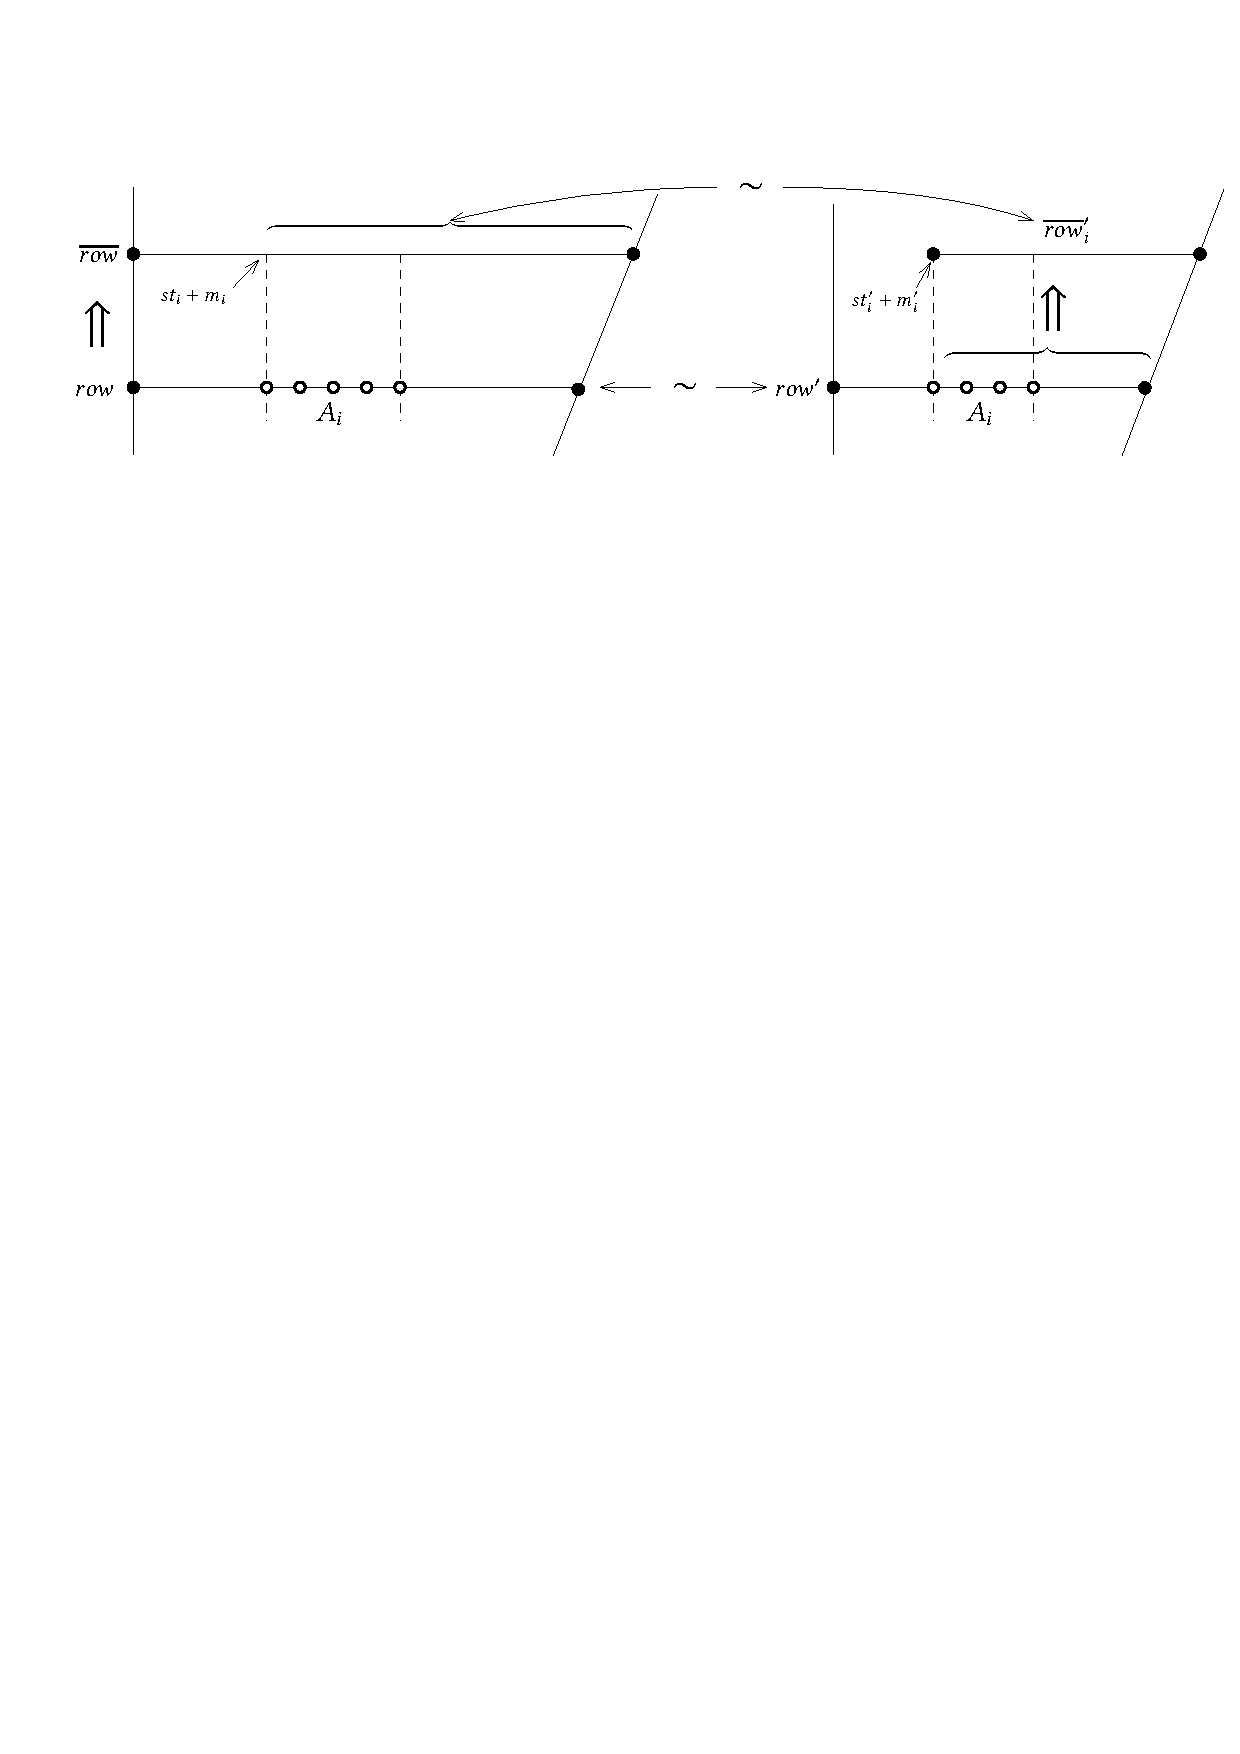
\includegraphics{Chaps/ICALP_D/generat}}
    \caption{Illustration of the properties of $\orow'_i$.}\label{fig:generat}
\end{sidewaysfigure}

The base case for $i=0$ is omitted, as it is just a simplification of the inductive step.
Let us consider $i\geq 1$. By the inductive hypothesis, we have $\orow'_{i-1}\sim \orow(0, st_{i-1}+m_{i-1})$ (hence in particular $\lst(\orow'_{i-1})=\orow(st_{i-1}+m_{i-1})$, where $\lst(\row)$ denotes the last atom of $\row$) and $\row'(0, st_{i-1}'+m_{i-1}'-1)\rownext \orow_{i-1}'$.
We consider three cases, corresponding to the cases of the definition of $\orow_i'$.
\begin{itemize}
	\item $m_i=m_i'$. Then $\orow'_i = \orow'_{i-1} \cdot \orow(st_i+1, st_i+m_i)$ is a $\varphi$-row. If $\lst(\orow'_{i-1})\neq (\orow(st_i+1))$, then it immediately follows that $\orow'_i\sim \orow(0, st_{i}+m_{i})$. 
	Conversely, if $\lst(\orow'_{i-1})=\orow(st_i+1)=\orow(st_{i-1}+m_{i-1})$, then $\orow(st_i+1)$ is reflexive. By Lemma~\ref{lem:rank0}, $\orow(st_i+1)=\ldots = \orow(st_i+m_i)$. It follows that $\orow'_i\sim \orow(0, st_{i}+m_{i})$, because we append to $\orow'_{i-1}$ exactly $\orow(st_i+1, st_i+m_i)$ (note that either $\orow(st_{i-1}+m_{i-1})$ already exceeded its rank in $\orow(0, st_{i-1}+m_{i-1})$ and so did $\lst(\orow_{i-1}')$ in $\orow_{i-1}'$, or the ranks of $\orow(st_{i-1}+m_{i-1})$ in $\orow(0, st_{i-1}+m_{i-1})$ and of $\lst(\orow_{i-1}')$ in $\orow_{i-1}'$ were equal).
	Moreover, in both cases, $\row'(0, st_i'+m_i'-1)\rownext \orow_i'$ by definition of $\genDphi$, as $\row'(st'_i)=\row(st_i)=A_i$ (recall that $\row\sim\row'$). 
	
	\item $\rank(A_i)<m'_i<m_i$. Then $\orow'_i = \orow'_{i-1} \cdot \orow(st_i+1, st_i+m'_i)$ is a $\varphi$-row. 
	First, we have $\row'(0, st_i'+m_i'-1)\rownext \orow_i'$ by definition of $\genDphi$, as $\row'(st'_i)=\row(st_i)=A_i$. 
	By Lemma~\ref{lem:rank}, being $\rank(A_i)<m_i$, there exists $st_i+1\leq k\leq st_i+m_i$ such that $\orow(k)$ exceeds its rank in $\orow(st_i+1, st_i+m_i)$, $\orow(k)=\ldots =\orow(st_i+m_i)$, and $k\leq st_i+1+\rank(A_i)$. We first note that, being $1+\rank(A_i)\leq m'_i$, we have $k\leq st_i+m'_i$, thus the atom $\orow(k)$ is present in the block $\orow(st_i+1, st_i+m'_i)$ of $\orow'_i$. 
	By Lemma~\ref{lem:rank}, being also $\rank(A_i)<m'_i$, we have that the atom $\orow(k)$ exceeds its rank in the block  $\orow(st_i+1, st_i+m'_i)$ of $\orow'_i$ as well. Thus $\orow'_i\sim \orow(0, st_i+m_i)$.
	
	\item $\rank(A_i)<m_i<m'_i$. Then $\orow'_i = \orow'_{i-1} \cdot \orow(st_i+1, st_i+m_i) \cdot (\orow(st_i+m_i))^{m'_i-m_i}$. By Lemma~\ref{lem:rank}, being $\rank(A_i)<m_i$, there exists $st_i+1\leq k\leq st_i+m_i$ such that $\orow(k)$ is reflexive, it exceeds its rank in $\orow(st_i+1, st_i+m_i)$, and $\orow(k)=\ldots =\orow(st_i+m_i)$.
	First we observe that $\orow'_i$ is a $\varphi$-row, being $\orow(st_i+m_i)$ reflexive. Then
	the atom $\orow(k)$ is (trivially) also present in the block $\orow(st_i+1, st_i+m_i)$ of $\orow'_i$. As a consequence $\orow'_i\sim \orow(0, st_i+m_i)$. Moreover, $A_i\, \orow(st_i+m_i) \genDphi \orow(st_i+m_i)$ (as $\orow(st_i+m_i)$ is reflexive), therefore $\row'(0, st_i'+m_i'-1)\rownext \orow_i'$.
	%	
	\qedhere
\end{itemize}
%This concludes the proof the theorem.
\end{proof}


The following result arranges the equivalence classes $\Rows^\sim$ in a graph $G_{\varphi \sim}$.
%
\begin{definition}\label{def:equivalencegraph}
Let $\varphi$ be a $\hsDhom$ formula. The \emph{$\varphi\!\sim$graph} of $\varphi$ is defined as $G_{\varphi \sim}=(\Rows^\sim,\rownext)$.
\end{definition}

The next theorem reduces the problem of SAT checking for a $\hsDhom$ formula $\varphi$ over finite linear orders (equivalent, by Proposition~\ref{prop:satiffcompass}, to deciding if there is a homogeneous fulfilling compass $\varphi$-structure that features $\varphi$) to a reachability problem in the $\varphi\!\sim$graph, allowing us to determine the computational complexity of the former problem.
%
\begin{theorem}\label{thm:path_iff_sat}
Given a $\hsDhom$ formula $\varphi$, there exists a homogeneous fulfilling compass $\varphi$-structure $\cG=(\bbP_\bbD, \cL)$ that features $\varphi$
if and only if there exists a path  in $G_{\varphi \sim}=(\Rows^\sim,\rownext)$
from some class $[\row]_\sim\in\Rows^\sim$ to some class $[\row']_\sim\in\Rows^\sim$ such that
\begin{enumerate}
    \item there exists $row_1\in[\row]_\sim$ with $|row_1|=1$, and
    \item there exist $row_2\in[\row']_\sim$ and $0\leq i<|row_2|$ such that $\varphi\in row_2(i)$.
\end{enumerate}
\end{theorem} 
%
\begin{proof}
Preliminarily we observe that, in (1.), if $|row_1|=1$, then $\{row_1\}=[\row]_\sim$; moreover, in (2.), if for $row_2\in[\row']_\sim$ and $0\leq i<|row_2|$ we have that $\varphi\in row_2(i)$, then for any $row_2'\in[\row']_\sim$, there is $0\leq i'<|row_2'|$ such that $\varphi\in row_2'(i')$.

($\Rightarrow$) 
Let us consider a homogeneous fulfilling compass $\varphi$-structure $\cG=(\bbP_\bbD, \cL)$ that features $\varphi$.
By Lemma~\ref{lem:compas_implies_row} and \ref{lem:row_successor}, 
$\cL(0,0) \rownext \allowbreak  \row_1 \rownext \cdots\linebreak \rownext \row_{\max(\mathpzc{S})}$. Thus
there exist two indexes $0\leq j\leq \max(\mathpzc{S})$ and $0\leq i<|row_j|$ for which $\varphi \in \row_j(i)$. 
By Definition~\ref{def:row_class_suc}, we get that $[\cL(0,0)]_\sim \rownext \allowbreak  [\row_1]_\sim \rownext \cdots \rownext [\row_{j}]_\sim$ is a path in $G_{\varphi \sim}$; it is immediate to check that it fulfills requirements (1.) and (2.).

($\Leftarrow$) Let us assume that there exists a path $[\row_0]_\sim 
\rownext \cdots \rownext [\row_{m}]_\sim$ in $G_{\varphi\sim}=\allowbreak (\Rows^\sim, \rownext)$
for which $|\row_0| = 1$ and there exists $i$ such that $\varphi\in \row_m(i)$. 
By applying repeatedly Lemma~\ref{lem:row_class_suc}
we get that there exists a sequence 
$\row'_0 \rownext \cdots \rownext \row'_{m}$ of $\varphi$-rows where $\row'_0 =\row_0$,
for every $0\leq j\leq m$, $\row'_j\in [\row_j]_\sim$,
and there exists $i'$ such that $\varphi\in \row_m'(i')$.
%
We observe that, by Definition~\ref{def:rownext},
$|\row_j'|=|\row_{j-1}'|+1$
 for $1\leq j \leq m$
and, since $|\row'_0|=1$, we have $|\row_{j}'|= j + 1$. 
%
Let us now define $\cG=(\bbP_\bbD, \cL)$ where $\mathpzc{S}= \{0,\ldots, m\}$ and
$\cL(x,y)=\row_y'(y-x)$ for every $0\leq x\leq y\leq m$.
By Lemma~\ref{lem:row_successor}, $\cG$ is a fulfilling homogeneous compass $\varphi$-structure.
Finally, since $\varphi\in \row_m'(i')$, $\cG$ features $\varphi$.
\end{proof}

The size of $G_{\varphi\sim}=(\Rows^\sim,\rownext)$ is bounded by $|\Rows^\sim|^2$, which is exponential 
in $|\varphi|$. However, 
it is possible to (non-deterministically) perform a reachability in $G_{\varphi \sim}$ by using space \emph{logarithmic} in $|\Rows^\sim|^2$.


\begin{algorithm}[b]
\begin{algorithmic}[1]
\caption{\texttt{SAT}$(\varphi)$}\label{NDAlgo}
%
    \State{$M\gets 2^{3|\varphi|^2}$, $step\gets 0$ and $\row\gets A$ for some atom $A\in \Atoms$ with  $\reqD(A)=\emptyset$}
    \If{there exists $0\leq i<|\row|$ such that $\varphi\in \row(i)$}
        \State{\textbf{return} ``satisfiable''}
    \EndIf
    \If{$step = M-1$}
        \State{\textbf{return} ``unsatisfiable''}
    \EndIf
    \State{Non-deterministically generate a $\varphi$-row $\row'$ and check that $\row \rownext \row'$}
    \State{$step \gets step +1$ and $\row \gets\row'$}
    \State{Go back to line 2}
%
\end{algorithmic}
\end{algorithm}

The \emph{non-deterministic} procedure \texttt{SAT}$(\varphi)$ in Algorithm~\ref{NDAlgo} exploits this fact in order to decide the satisfiability 
of a $\hsDhom$ formula $\varphi$, by using only a working space \emph{polynomial} in $|\varphi|$: it searches for a suitable path in $G_{\varphi \sim}$, namely  $[\row_0]_\sim \rownext \cdots \allowbreak \rownext [\row_{m}]_\sim$, where $\row_0 =A$ for $A\in \Atoms$ with  $\reqD(A)=\emptyset$, $m< M$, and $\varphi\in \row_m(i)$ for $0\leq i<|\row_m|$. At the $j$-th iteration of line 6., $\row_{j}$ is non-deterministically generated, and it is checked whether $\row_{j-1}\rownext\row_{j}$.
The procedure terminates after at most $M$ iterations, where $M$ is the maximum possible length of a simple path in $G_{\varphi\sim}$.

The working space used by the procedure is polynomial:
$M$
and $step$ (which ranges in $[0,M-1]$) can be encoded 
in binary with $\lceil \log_2 M \rceil +1=O(|\varphi|^2)$ bits.  
At each step, we need to keep track of two $\varphi$-rows at a time, the current one, $\row$, and its successor, $\row'$: each $\varphi$-row can be represented as a sequence of at most $2|\varphi|$ (distinct) atoms,
each one with an exponent that, by construction, cannot exceed $M$. 
Moreover, each $\varphi$-atom $A$ can be represented using exactly $|\varphi|$ bits (for each
$\psi \in \CL(\varphi)$, we set a bit to 1 if $\psi\in A$, and to 0 if $\neg\psi\in A$). Hence a $\varphi$-row can be encoded using $2|\varphi|\cdot(|\varphi|+\lceil \log_2 M \rceil +1)=O(|\varphi|^3)$ bits. 
%
Finally, the condition $\row \rownext \row'$ can be checked
by $O(|\varphi|^2)$ bits of space once we have guessed $\row'$. 
This analysis entails the following result (we recall that $\NPsp=\Psp$).
%
\begin{theorem}\label{thm:pspace}
The SAT problem for $\hsDhom$ formulas over finite linear orders is in $\Psp$.
\end{theorem} 


We now outline which are the modifications to the previous concepts needed for proving the 
decidability of SAT for $\hsDhom${} with the strict relation $\ssubint$, in place of $\subint$.
It is sufficient to replace the definitions
of $\genDphi$,  $\varphi$-$\row$ and $\rownext$
with the following ones. 
For the sake of simplicity, we introduce a dummy atom $\boxdot$, for which we assume $\reqD(\boxdot)=\obsD(\boxdot)=\emptyset$.

\begin{definition}\label{def:d_generatorS}
Given four $\varphi$-atoms $A_1, A_3,A_4\in\Atoms$ and $A_2\in\Atoms\cup\{\boxdot\}$, we say that 
$A_4$ is \mbox{$\Dphi\ssubint$-generated} by $A_1,A_2,A_3$,
written $A_1,A_2, A_3\genDphiS A_4$, if:  
\begin{itemize}
    \item $A_4\cap\AP = A_1 \cap A_3 \cap \AP$ and 
    \item $\reqD(A_4)=\reqD(A_1)\cup \reqD(A_3) \cup \obsD(A_2 )$.
\end{itemize}
\end{definition}
The idea of this definition is that, if an interval $[x,y]$, with $x<y$, is labeled by $A_4$, and the three subintervals $[x,y-1]$, $[x+1,y-1]$, and $[x+1,y]$ by $A_1$, $A_2$, $A_3$, respectively, we want $A_1,A_2, A_3\genDphiS A_4$. In particular, if $x=y-1$, then $A_2=\boxdot$ (because $[x+1,y-1]$ is not a valid interval). Note that only $[x+1,y-1]\ssubint[x,y]$, hence we want $\obsD(A_2)\subseteq\reqD(A_4)$; moreover, since the requests of $A_1$ and $A_3$ are fulfilled by a strict subinterval of $[x,y]$, it must be $\reqD(A_1)\subseteq\reqD(A_4)$ and $\reqD(A_3)\subseteq\reqD(A_4)$. 

\begin{definition}\label{def:rowS}
A $\varphi$-$\ssubint$-row is a finite sequence of $\varphi$-atoms \[\row=A_0^{m_0}\cdots A_n^{m_n},\]
%(where $A^m$ stands for $m$ repetitions of $A$) 
such that for each $0\leq i \leq n$, we have $m_i>0$, and for each $0\leq j<i$, it holds $\reqD(A_j) \subseteq \reqD (A_i)$, $A_i \neq A_j$, and $(A_j\cap \AP)\supseteq (A_i\cap \AP)$.
 Moreover, $\reqD(A_0)=\emptyset$.
\end{definition}

\begin{definition}\label{def:rownextS}
Given two $\varphi$-rows $\row$ and $\row'$, we say that $\row'$ is a successor
of $\row$, written as $\row\rownextS\row'$, if $|\row'| = |\row| +1$, and for all $0\leq i < |\row|$,
$\row(i)\row(i-1)\row'(i) \genDphiS \row'(i+1)$, where we assume 
$\row(i-1)=\boxdot$ if $i=0$. 
\end{definition}

% We conclude the section by outlining how it is possible to prove that satisfiability for $\hsDhom${} over finite linear orders is a $\Psp$-complete problem (under both the \emph{strict} and \emph{proper} semantic variants).
% %
% The argument is straightforward, and proceeds by a reduction from the $\Psp$-complete \emph{problem of satisfiability of a quantified Boolean formula (QBF)}~\cite{Stockmeyer:1973:WPR:800125.804029},
% %%
% which is an expression of the form $\theta = Q_1p_1\cdots Q_n p_n \psi$,
% where  $\psi$ is a (quantifier-free) formula of Boolean logic over the variables $\{p_1,\ldots,p_n\}$, and for all
% $1\leq i \leq n$, $Q_i$ is either $\forall$ or $\exists$.

% Intuitively, $\theta$ is true iff we can find a \emph{tree} such that: $(i)$ the root is associated with $\theta$,
% $(ii)$ if a node is associated with some $Q_jp_j\cdots Q_n p_n \phi$, with $1\leq j\leq n$, and $Q_j=\exists$ (resp., $Q_j=\forall$), then it has exactly a child (resp., two children) associated with $Q_{j+1}p_{j+1}\cdots Q_n p_n (\phi\{p_j\to\top\})$, or (resp., and) with $Q_{j+1}p_{j+1}\cdots Q_n p_n (\phi\{p_j\to\bot\})$---$\phi\{p_j\to *\}$ is $\phi$ where all the occurrences of $p_j$ have been replaced by the constant $*$, for $*=\top,\bot$---$(iv)$ all the leaves are associated with \emph{true} variable-free Boolean formulas over the constants $\top,\bot$.

% \begin{figure}[tb]
%     \resizebox{\textwidth}{0.7\height}{\input{QBFTree}}
%     \caption{\label{fig:hard_example} A tree witnessing the satisfiability of a QBF formula, encoded by an interval model}
% \end{figure} 

% It is then possible to embed a tree over a linear order: we can find a $\hsDhom$-formula $\psi_\theta$ such that, if satisfied by a homogeneous interval model, forces it to correctly encode a tree witnessing the satisfiability of $\theta$.
% %
% For example, if the QBF formula is
% $
% \theta=\forall p_1\exists p_2 \forall p_3 \exists p_4( (p_1 \vee p_2) \wedge (\neg p_1 \vee \neg p_2) \wedge (p_3 \vee p_4) \wedge (\neg p_3 \vee \neg p_4)  )
% $,
% a homogeneous interval model encoding a tree for $\theta$ is shown in Figure \ref{fig:hard_example}, where the auxiliary letter $sub_i^\top$ (resp., $sub_i^\bot$) ``forces'' $p_i$ to be true (resp., false) on every interval over which it holds. 
% %

We will come back to SAT later, showing the $\Psp$-completeness of such problem  (under both the \emph{strict} and the \emph{proper} semantic variants). In the next section, we will consider MC for $\hsDhom$.
